\documentclass[10pt]{beamer}

\usetheme[progressbar=frametitle]{metropolis}

\usepackage[T1]{fontenc}
\usepackage{newunicodechar}
%\usepackage[utf8]{inputenc}

\usepackage{subcaption}
\usepackage{adjustbox}
\usepackage{booktabs}
\usepackage[scale=2]{ccicons}

% For pseudo codes
\usepackage{algorithm}
\usepackage[noend]{algpseudocode}
\makeatletter
\def\BState{\State\hskip-\ALG@thistlm}
\makeatother
%

\usepackage{multirow}
\usepackage[none]{hyphenat}
\usepackage{textcomp}
\usepackage{gensymb}
\sloppy 
%\usebackgroundtemplate


\usepackage{pgfplots}
\usepgfplotslibrary{dateplot}

\usepackage{xspace}
\newcommand{\themename}{\textbf{\textsc{metropolis}}\xspace}

\setbeamercolor{background canvas}{bg=white!20}

\title{A Style Based Generator Architecture for Generative Adversarial Networks}
\date{\regno}
\author{Vyshak Puthusseri}
\institute{MCA CET}


% logo of IPST 2019


\newcommand{\nologo}{\setbeamertemplate{logo}{}} % command to set the logo to nothing
\newcommand{\congress}{MCA CET}

% footer
\makeatletter
\setbeamertemplate{footline}
{
  \leavevmode%
  \hbox{%

  \begin{beamercolorbox}[wd=.9\paperwidth,ht=2.25ex,dp=1ex,center]{institute in head/foot}%
    \usebeamerfont{abstract}%
    \congress
  \end{beamercolorbox}%

  \begin{beamercolorbox}[wd=.1\paperwidth,ht=2.25ex,dp=1ex,right]{institute in head/foot}%
    \usebeamerfont{abstract} 
    \insertframenumber{} / \inserttotalframenumber\hspace*{1ex} 
  \end{beamercolorbox}}%
  
}
\makeatother




% Document begin %%%%%%%%%%%%%%%%%%%%%%%%%%%%%%%%%%%%%%%%%%%%%%%%%%%%%%%%%%%%%%%%%%%%
\begin{document}

\maketitle
%%%%%%%%%%%%%%%%%%%%%%%%%%%%%%%%%%%%%%%%%%%%%%%%%%%%%%%%%%%%%%




%%%%%%%%%%%%%%%%%%%%%%
{
\begin{frame}[fragile]{Introduction}

    \begin{itemize}
      \item Deep Learning 
      \item GAN : Generative Adversarial Network
      \item Style Transfer
      \item Style Based Generator Architecture for GAN
    \end{itemize}

\end{frame}
}

%%%%%%%%%%%%%%%%%%%%%%                                              About LTU
\begin{frame}[fragile]{Deep Learning - HOW?}
LTU  : 
\textbf{Linear Threshold Unit}\\
Building blocks of neural networks
Proposed by Warren McCulloch and Walter Pitts\\
Only a concept, No learning strategy

    \begin{figure}[ht]
      \hspace*{-1cm}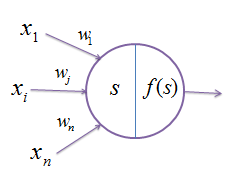
\includegraphics[width=0.5\linewidth]{ltu_image}
    \end{figure}
\end{frame}
%%%%%%%%%%%%%%%%%%%%%%                                          About Perceptron
\begin{frame}[fragile]{Deep Learning - HOW?}

Perceptron
    \begin{itemize}
        \item LTU + Learning rule .
\pause        
        \item Works only for binary classification
    \end{itemize}
    \begin{figure}[ht]
      \hspace*{-1cm}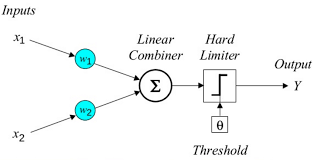
\includegraphics[width=0.5\linewidth]{ltu}
    \end{figure}
\end{frame}
%%%%%%%%%%%%%%%%%%%%%%                                          About MLP
\begin{frame}[fragile]{Deep Learning - HOW?}
    Multilayer Perceptron
    \begin{itemize}
        \item Multiple perceptrons are stacked side by side and on top
\pause        
        \item Activation function : Sigmoid
    \end{itemize}
    \begin{figure}[ht]
      \hspace*{-1cm}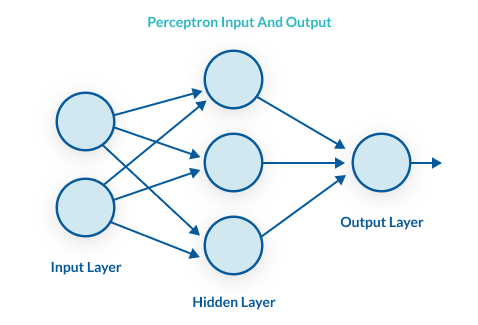
\includegraphics[width=0.5\linewidth]{mlp}
    \end{figure}
\end{frame}

%%%%%%%%%%%%%%%%%%%%%%                                          About Deep neural network
\begin{frame}[fragile]{Deep Learning - HOW?}
    Deep Neural Network \\ 
    If there is only one hidden layer
    \begin{figure}[ht]
      \hspace*{-1cm}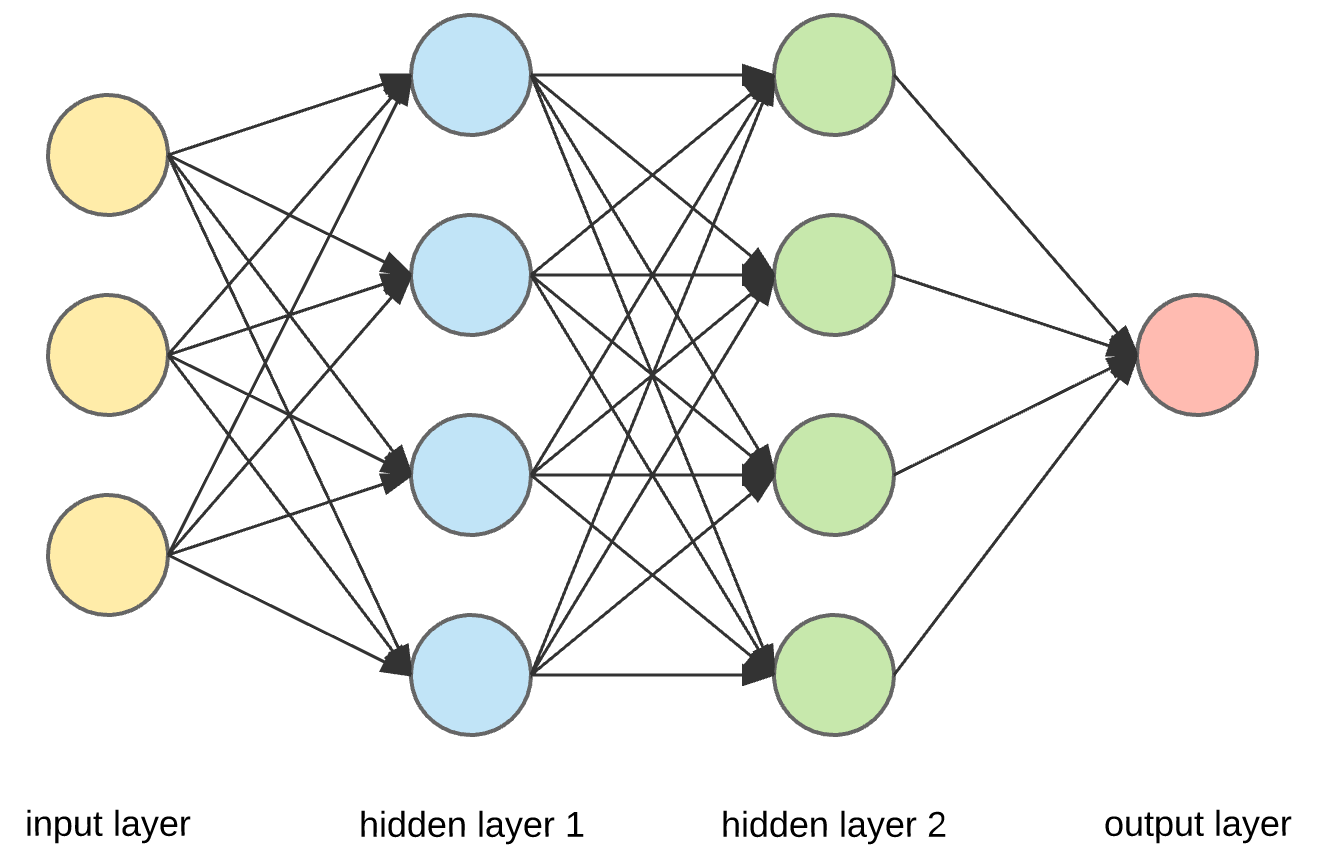
\includegraphics[width=0.5\linewidth]{dnn}
    \end{figure}
Learning Weights of a deep neurral networks is called as \textbf{deep learning}
\end{frame}

%%%%%%%%%%%%%%%%%%%%%%                                          About Convolutional layer
\begin{frame}[fragile]{Convolutional Neural Networks}
    Why \\ 
    \begin{figure}[ht]
      \hspace*{-1cm}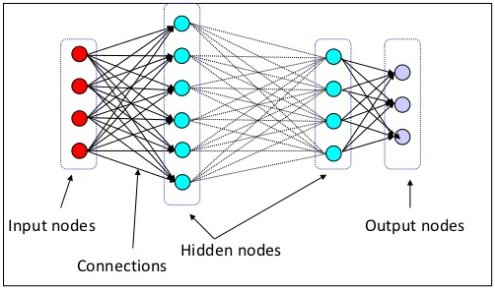
\includegraphics[width=0.5\linewidth]{conv1} \\
      \hspace*{-1cm}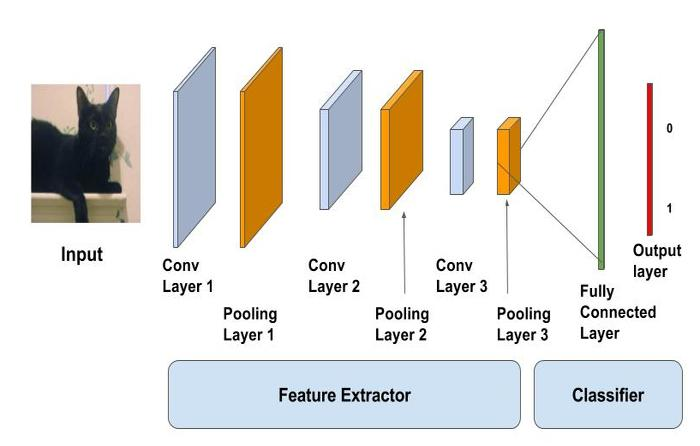
\includegraphics[width=0.5\linewidth]{conv2}
    \end{figure}
Learning Weights of a deep neurral networks is called as \textbf{deep learning}
\end{frame}

%%%%%%%%%%%%%%%%%%%%%%%%%%%%%%%%%%%%%%%%%%%%%%%%%%%%%%%%%%%%%%%%%%%%%%%%%%%%%%%%%%%%%%%%

%%%%%%%%%%%%%%%%%%%%%%                                          About Style Transfer
\begin{frame}[fragile]{Neural Style Transfer}
   Style transfer relies on separating the content and style of an image. 
   \\
   Given one content image and one style image, we aim to create a new, target image which should contain our desired content and style components:
    \begin{itemize}
        \item objects and their arrangement are similar to that of the content image (feature reconstruction)
        \item style, colors, and textures are similar to that of the style image (texture synthesis)
    \end{itemize}

\end{frame}


%%%%%%%%%%%%%%%%%%%%%%                                         
\begin{frame}[fragile]{Neural Style Transfer}
    \begin{equation}
        content.image + style.image =  new.image with style.transfered
    \end{equation}
    \begin{figure}[ht]
      \hspace*{-1cm}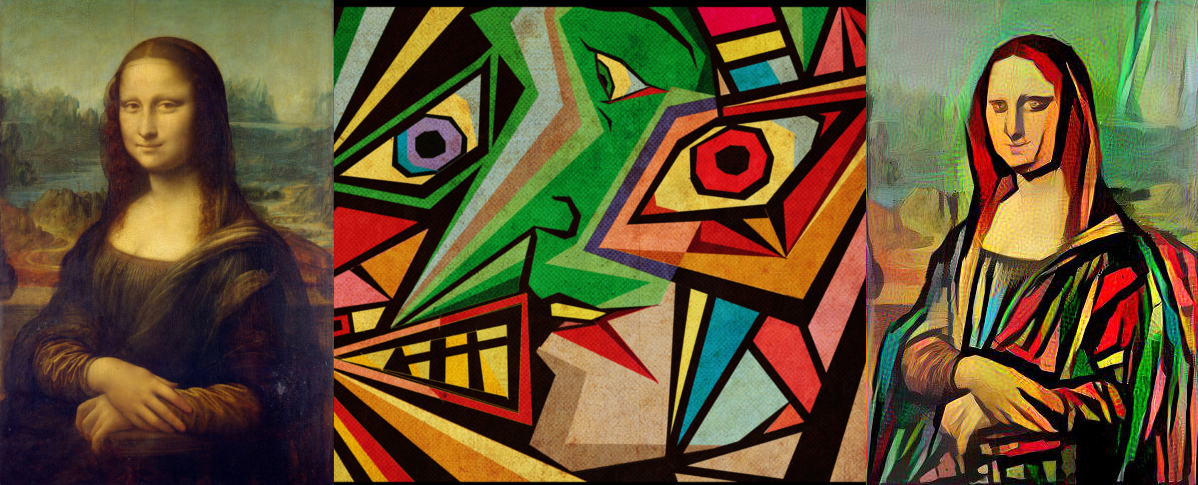
\includegraphics[width=0.5\linewidth]{styletransfer} \\
      \hspace*{-1cm}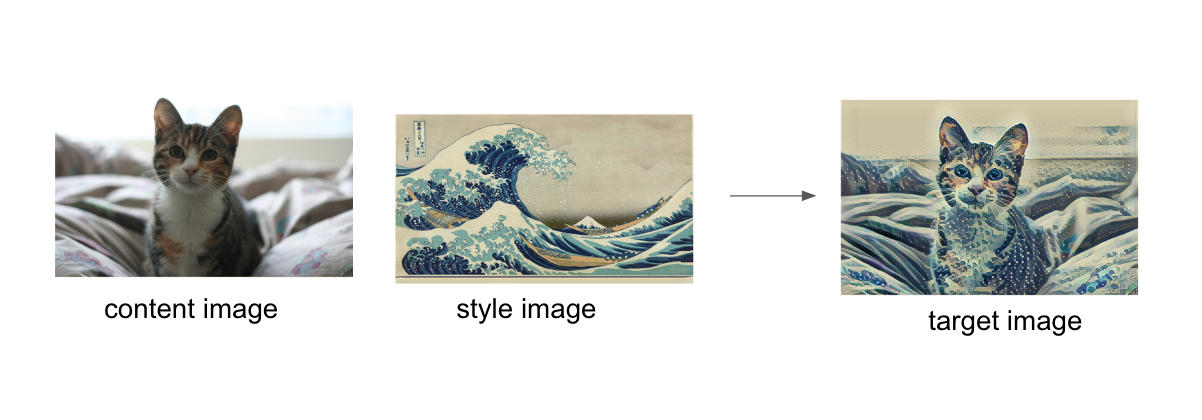
\includegraphics[width=0.7\linewidth]{styletransfercat} 
    \end{figure}
    https://github.com/puthusseri/styleTransfer.git
\end{frame}


%%%%%%%%%%%%%%%%%%%%%%%%%%%%%%%%%%%%%%%%%%%%%%%%%%



%%%%%%%%%%%%%%%%%%%%%%                                          About GAN                    
\begin{frame}[fragile]{Generative Adversarial Network}
 GANs are generative models: they create new data instances that resemble your training data. \\
 eg: images that look like photographs of human faces, even though the faces don't belong to any real person.
     \begin{figure}[ht]
      \hspace*{-1cm}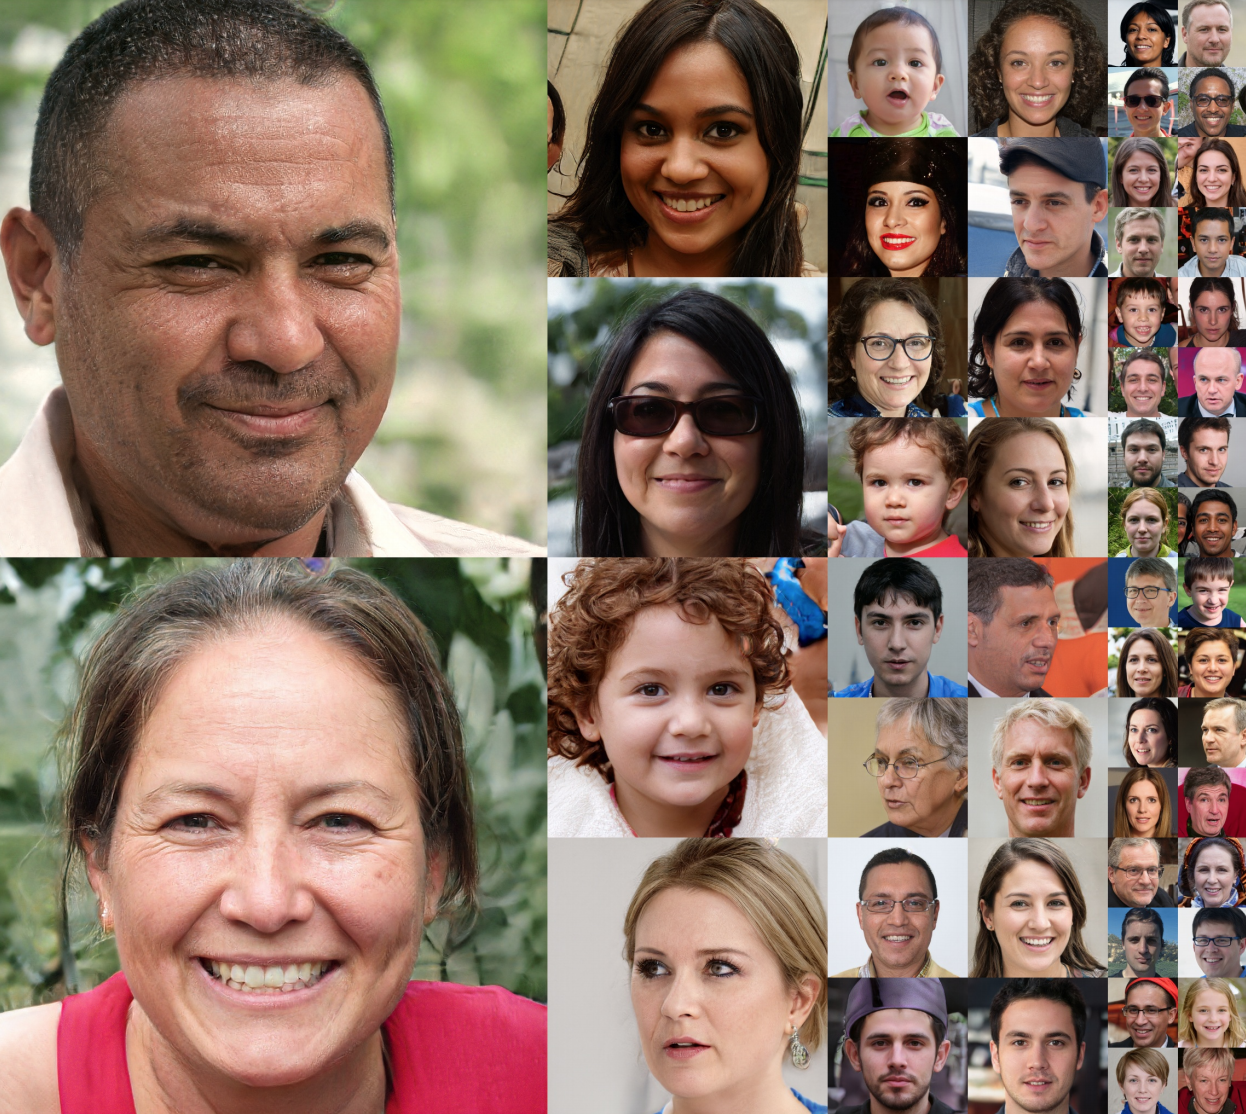
\includegraphics[width=0.5\linewidth]{ganhumans} 

    \end{figure}
\end{frame}

%%%%%%%%%%%%%%%%%%%%%%                                          About GAN Applications                   
\begin{frame}[fragile]{GAN : Applications}

    \begin{itemize}
        \item Image to image translation (in unsupervised way)
        \item blue prints to real image
        \item photo to cartoon (Facebook AI research)
        \item photo of day to night (NVIDIA Research)
        \item Creating stimulated training set (eg : face recognition problem)
        \item for imitaion learning
    \end{itemize}
\end{frame}

%%%%%%%%%%%%%%%%%%%%%%                                          About GAN Overview                   
\begin{frame}[fragile]{GAN : Overview}
 GANs has two parts: \\
    \begin{itemize}
        \item The generator : learns to generate plausible data. The generated instances become negative training examples for the discriminator.

        \item The discriminator: learns to distinguish the generator's fake data from real data. The discriminator penalizes the generator for producing implausible results.
    \end{itemize}
\end{frame}


%%%%%%%%%%%%%%%%%%%%%%                                          About GAN Training                   
\begin{frame}[fragile]{GAN : Training}
     \begin{figure}[ht]
         \hspace*{-1cm}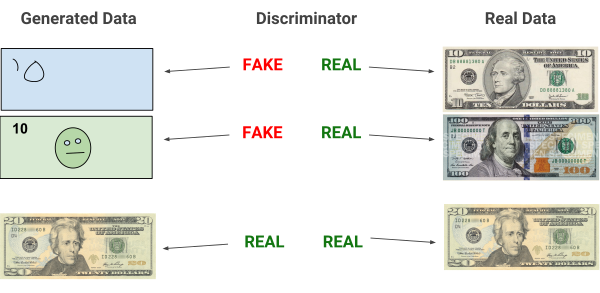
\includegraphics[width=0.7\linewidth]{gantrain} \\ \\ \\ \\ \\ 


    \end{figure}
\end{frame}

%%%%%%%%%%%%%%%%%%%%%%                                          About GAN Architecture                   
\begin{frame}[fragile]{GAN : Architecture}
     \begin{figure}[ht]
         \hspace*{-1cm}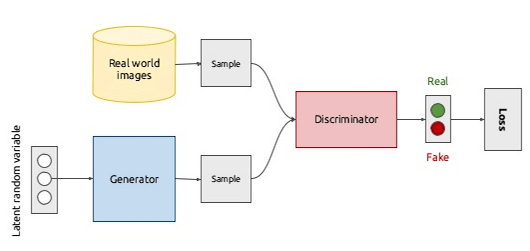
\includegraphics[width=0.7\linewidth]{ganarchitecture.png} \\ \\ \\ \\ \\ 
    \end{figure}
\end{frame}
%%%%%%%%%%%%%%%%%%%%%%%%%%%%%%%%%%%%%%%%%%%%%%%%%%%%%%%%%%%%%%%%%%%%%%
%%%%%%%%%%%%%%%%%%%%%%                                          About Style Based GAN                   
\begin{frame}[fragile]{Style Based GAN}
        \begin{itemize}
        \item Introduced by NVIDIA 
        \item Improved the efficiency of GAN by improving the generator
        \item Introduced new automated metrics - perceptual path length and linear seperability
        \item Result was  : new dataset Flickr Face HQ (FFHQ) of size 2.56 TB
    \end{itemize}

\end{frame}

%%%%%%%%%%%%%%%%%%%%%%                                          About Style Based Generator                   
\begin{frame}[fragile]{Style Based Generator}
        \begin{itemize}
        \item The weights are studied through the 8 layer affine transformation.
        \item Feature maps are normalized using AdaIN
        \item Generate \textit{stochastic details} by introducing the explicit noise for each layer.
        \item Final resulting feature maps are passd to the discriminator.
    \end{itemize}

\end{frame}

%%%%%%%%%%%%%%%%%%%%%%                           About Style Based Generator Architecture                   
\begin{frame}[fragile]{Style Based Generator : Architecture}
     \begin{figure}[ht]
         \hspace*{-1cm}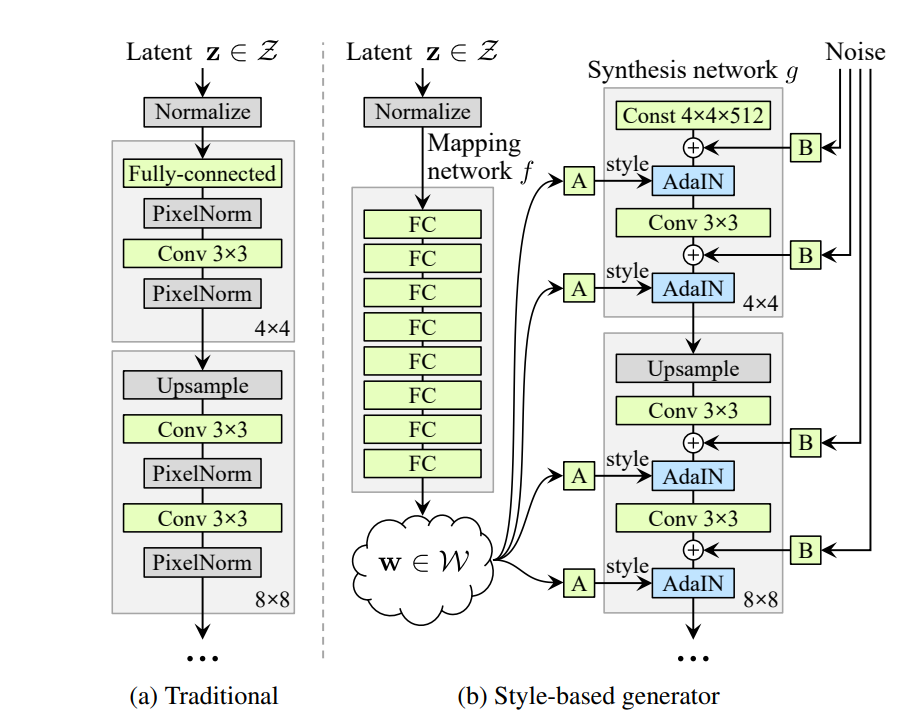
\includegraphics[width=0.9\linewidth]{styleganarchitecture.png} \\ \\ \\ \\ \\
    \end{figure}
\end{frame}

%%%%%%%%%%%%%%%%%%%%%%                                          About Style Based Image Quality                   
\begin{frame}[fragile]{Image Quality }
        \begin{itemize}
        \item Comparing with CELENA-HQ with FFHQ based on Frechet inception distances (FID) , a great improvement happens
        \item Used truncation trick
        \item Used 26.3M parameters for training
        \item Generated image is of 1024 * 1024 resolution
    \end{itemize}

\end{frame}

%%%%%%%%%%%%%%%%%%%%%%%%%%%%%%%%%%%%%%%%%%%%%%%%%%%%%%%%%%%%%%%%%%%%%%

%%%%%%%%%%%%%%%%%%%%%%                                  About Style Based generator Properties  1                 
\begin{frame}[fragile]{Style Based Generator : Properties }
        \begin{itemize}
        \item Style mixing - mixing regularization
    \end{itemize}
    \begin{figure}[ht]
         \hspace*{-1cm}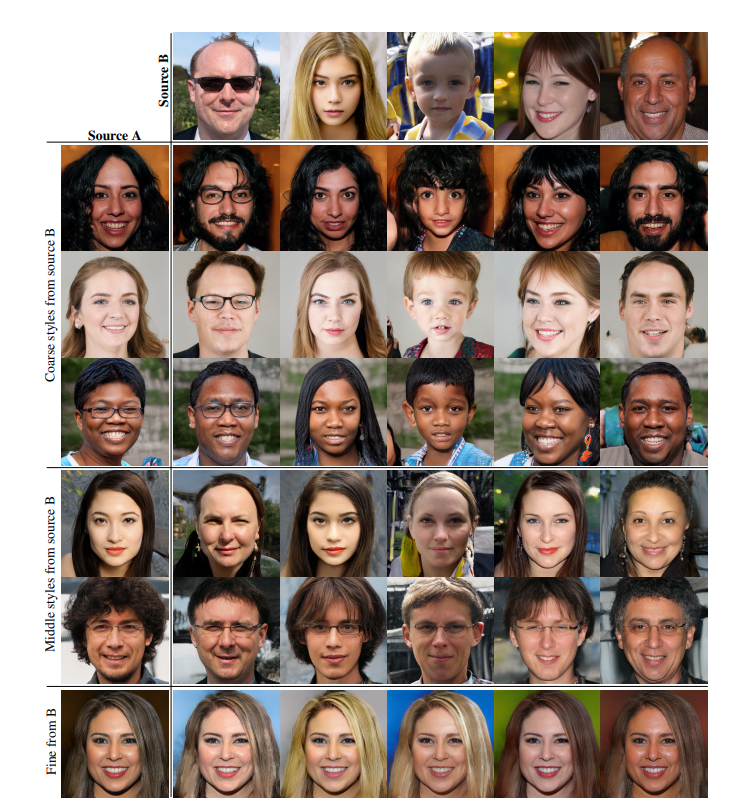
\includegraphics[width=0.6\linewidth]{stylemixing.png} \\ \\ \\ \\ \\
    \end{figure}

\end{frame}

%%%%%%%%%%%%%%%%%%%%%%                                  About Style Based generator Properties  2                
\begin{frame}[fragile]{Style Based Generator : Properties }
        \begin{itemize}
        \item Stochastic variation
    \end{itemize}
    \begin{figure}[ht]
         \hspace*{-1cm}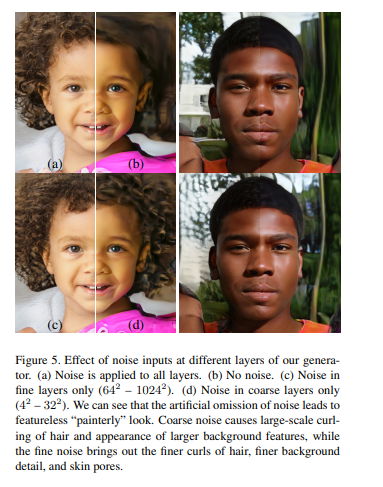
\includegraphics[width=0.7\linewidth]{stochasticvariation.png} \\ \\ \\ \\ \\
    \end{figure}

\end{frame}

%%%%%%%%%%%%%%%%%%%%%%%%%%%%%%%%%%%%%%%%%%%%%%%%%%%%%%%%%%%%%%%%%%%%%%
\section{Conclusions}


%%%%%%%%%%%%%%%%%%%%%%%%%%%%%%%%%%%%%%%%%%%%%%%%%%%%%%%%%%%%%%

\begin{frame}[standout]
  Thank you \\ Questions?
\end{frame}

\end{document}
